\subsection{Related Technologies}
It is almost always beneficial for developers of a product to research and study related or similar products, as well as products related to their product's subsystems, in detail to gain a better understanding of how a subsystem can operate, and how subsystems can integrate with each other to form a cohesive system. In this section, members of our team explore technologies and solutions related to our product and its various subsystems. Some of the technologies studied below can be, and most likely will be integrated into our final product.

\subsubsection{Ocean insight: Ocean ST NIR Microspectrometer}
Ocean Insight is a local manufacturer of high-end, low size, weight, and power spectrometers. The ST NIR Microspectrometer is about 40 cubic centimeters in volume with a scan speed of 10ms, a signal to noise ratio of 190:1, and a spectral resolution of 2.2nm. Its spectral range is from 645nm to 1085nm, and it was specifically designed to be integrated into larger systems for customers who were interested in a flexible, low-cost design. Added to that, the system is rugged, and offers a variable slit input size, increasing its flexibility even further. While the designs are proprietary, this system serves as a benchmark for what can be achieved by the industry, and no doubt there are major design changes that can be made to achieve a similar result for the application intended for the Auto Garden Bed. That being said, the selling price for one is \textdollar1,750.

\begin{figure}[H]
    \caption{Ocean ST NIR Microspectrometer}
    \centering
    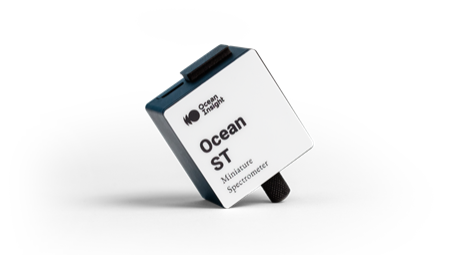
\includegraphics[width=0.5\textwidth]{images/3-2-1Pic.png}
\end{figure}

\subsubsection{AgroCares Nutrient Soil Scanner}

AgroCares offers a Near Infrared Spectrometer specifically designed for Proximity Soil Sensing. Its spectral range is from 1300 to 2500nm and it uses Micro Electrical Mechanical Systems or MEMS to capture EM Waves reflecting off the soil. The real value of the product is in its wireless communications system. The device uses Bluetooth 4.0 to send data to a cloud data center. There, spectrographs of large data sets of soil with known nutrient contents are compared with the reading, cutting out the need for on-sight calibration. The system is handheld and uses eight tungsten halogen bulbs to blast the soil with energy. This light is collected in an extremely small area, sampling 65 squared millimeters. It would be worth researching to see if the Tungsten bulbs were linked to the 1300 to 2500nm spectral range or if another probe and sensor would suffice.

\begin{figure}[H]
    \caption{AgroCares Nutrient Soil Scanner}
    \centering
    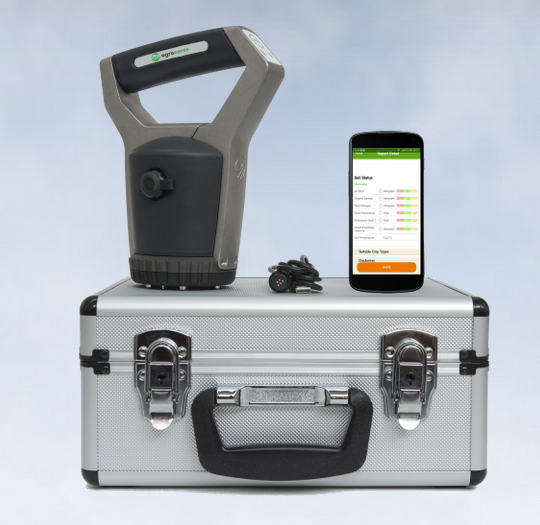
\includegraphics[width=0.5\textwidth]{images/3-2-2Pic.png}
\end{figure}

\subsubsection{DIY Webcam Diffraction Grating Spectrometer}\label{sec:DIYTransmissionGratingSpectrometer}

Physics Open Lab is a blog posting site for do-it-yourself physics laboratory projects. This project makes use of a megapixel webcam and a 1000 line/mm transmissive diffraction grating. The megapixel sensor allows for “staring” scanning, which is used in conjunction with spectrograph software for identifying the wavelength bands as they spread out from the zero order transmission. The project offers some interesting ideas, from the use of open source spectroscopy software to the use of two dimensional spectral analysis. Unfortunately, the use of a transmission grating presents a major problem for this application. Transmission gratings output most of their optical power straight ahead, and they are difficult to separate as higher order groups. While the project results where impressive, it did not generate a single spectrograph past the 1um range, which is necessary to detect the Moisture Content of the Soil.

\begin{figure}[H]
    \caption{Webcam Transmission Grating Spectrometer}
    \centering
    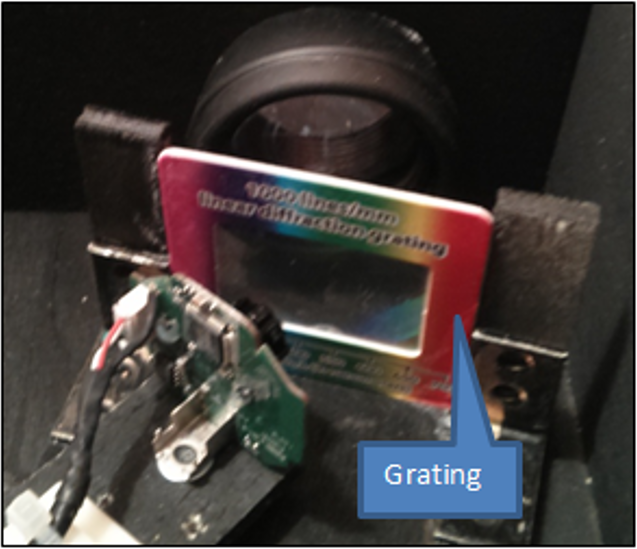
\includegraphics[width=0.5\textwidth]{images/DIYTransmissionGratingSpectrometer.png}
\end{figure}

\subsubsection{Proportional-integral-derivative Control}
Proportional-integral-derivative control (PID control) is a common control algorithm (espectially in industrial control systems) to allow a control loop to have reliable performance in a variety of conditions. Simply put, this algorithm allows a controller to receive an input and calculate a proportional output, accounting for error and rapid changes in the process. This algorithm may be useful to our application because it will allow the product to better control its facilities without user input.

The control function is defined in \autoref{eq:pid_controller}, where $u(t)$ is the control variable (e.g. the garden bed's water control solenoid), $K_p$, $K_i$, and $K_d$ are gain factors, and $e(t)$ (the error) is the different between a desired setpoint and measured process variable (e.g. the difference between the desired and current ounces of water dispensed).
\begin{equation}
    \label{eq:pid_controller}
    u(t) = K_pe(t) + K_i\int_{0}^{t}e(\tau) \, d\tau + K_d\frac{de(t)}{dt}
\end{equation}

\paragraph{Proportional Term} The proportional term of \autoref{eq:pid_controller} is $K_pe(t)$, hence referred to as the P-term. The P-term is proportional to the current error, and the gain $K_p$ determines the magnitude of the P-term. If the gain is too large, then the process variable will oscillate.

\paragraph{Integral Term} The integral term of \autoref{eq:pid_controller} is $K_i\int_{0}^{t}e(\tau) \, d\tau$, hence referred to as the I-term. This term accounts for previous values of $e(t)$ by taking the integral of the error, and the gain $K_i$ determines the magnitude of the I-term. The I-term aims to account for residual error in the control loop.

\paragraph{Derivative Term} The integral term of \autoref{eq:pid_controller} is $K_d\frac{de(t)}{dt}$, hence referred to as the D-term. The D-term aims to control future values of $e(t)$ by taking the derivative of the error, and the gain $K_d$ determines the magnitude of the D-term. This term acts to damp rapid changes in the control loop. Higher values of gain may make the control loop more sensitive to noise and lead to instability.

\subsubsection{Arduino Impletmentation of Microcontroller Internet Connection} Our team ultimately decided to implement a Texas Instruments microcontroller (detailed later) in the controls subsystem. This TI MCU contains an integrated network stack, and offers simple directions on connecting a compatible 2.4 GHz antenna. However, the one drawback our team did not expect was the relative abstractness, complication, and bureaucracy of creating programming with the tools required by TI. Between their proprietary distrobution of Eclipse, the libraries and SDKs required by the compiler, the configuratio of the compiler and linker, and the relative abstractness and complication of their libraries located in the SDK, the TI MCU is difficult to work with if the developer does not have pervious experience. In this section, Arduino's implementation is investigated and compared to our current TI MCU.

\paragraph{Arduino} Arduino is a microcontroller development board (integrating ATmega microcontrollers) distributor with a focus on hobbyists, especially entry-level developers. Compared to Texas Instruments, an industry-focused manufacturer, Arduino development has a very low bar to entry. Because of this, the fine granular control that may be required of an enterprise-level project is not present on Arduino boards---however, there are major advantages that make considering Arduino over TI worthwile:
\begin{itemize}
    \item Libraries are easy to implement
    \item The compiler and linker are relatively easy to configure compared to TI
    \item Large community following, support
    \item 3rd-party libraries are common and accessible
    \item Lower cost of components
    \item Easier to source components (in the year 2022)
    \item "Shields" (e.g. WiFi, GSM/GPRS, Bluetooth, GPS, motor controller, etc.) easily implementable
\end{itemize}
\paragraph{GSM/GPRS} One shield offered by Arduino is the \href{https://store.arduino.cc/products/arduino-mkr-gsm-1400}{Arduino MKR GSM 1400}, a 3G cellular network shield that enables SMS, voice, and internet connection. Arduino's library gives various "from scratch" examples and ample documentation on how to use different parts of its 1st-party \href{https://docs.arduino.cc/retired/archived-libraries/GSM}{GSM library}. For example, if one would like to connect a GSM network, it's as simple as including \texttt{GSM.h}, instantiating the \texttt{GSM} class (e.g. \texttt{GSM gsmAccess;}), and calling \texttt{begin()} (e.g. \texttt{gsmAcess.bein()}).

\paragraph{WiFi} Arduino offers shields like the \href{https://store.arduino.cc/products/arduino-mkr-wifi-1010}{Arduino MKR WiFi 1010}, as well as complete development boards like the \href{https://store.arduino.cc/products/arduino-uno-wifi-rev2}{Arduino Uno WiFi Rev2} with integrated WiFi modules. Just like the GSM library, Arduino's \href{https://www.arduino.cc/reference/en/libraries/wifi/}{WiFi library} is very easy to implement and use, and its documentation is wholly informative with class and function definitions and plenty of examples. For example, all one need do to connect to a network is detailed in the example in \autoref{fig:arduino_wifi_example}.

\begin{figure}[hbtp]
    \caption{Arduino WiFi code example}
    %\centering
    \label{fig:arduino_wifi_example}
    \begin{lstlisting}[language=c,frame=none,numbers=left,numbersep=-10pt,numberstyle=\tiny,basicstyle=\footnotesize\ttfamily]
        #include <WiFi.h>

        char ssid[] = "exampleNetwork";
        void setup() {
            while (status != WL_CONNECTED) {
                // Attempt to connect to SSID
                status = WiFi.begin(ssid);

                // Wait 10 seconds
                delay(10000);
            }

            // Once you reach here, you're connected
    \end{lstlisting}
\end{figure}

The user can go on to perform many different functions, with the limitation that they are either TCP or UDP bytestreams. This differs greatly from the TI CC3200's multifunctionality of being able to perform HTTP requests, Websockets, and many more on top of being able to take advantage of TCP and UDP bytestreams.